\chapter{Methodology and Implementation}
\label{ch:SC}
%\section{abvvv}
\par After extensive literature survey, it is found that Carla, TORCS, Airsim, SUMO are a few simulators which are considered for autonomous driving applications. Each of them has its own pros and cons. Carla and Airsim, being relatively new softwares, are more suitable for vision based driving and are known for their photo-realistic driving scenes which require higher graphic computations. SUMO does not have its RL capabilities very well developed. On the other hand TORCS simulator satisfies the requirements to implement this project. Hence, TORCS-1.3.7 in Ubuntu 16.04 OS with Python 3.5 with tensorflow and keras deep learning framework is used.
It is an open source, lightweight simulator software which is preferred due to its simplicity and variety of driving dynamics.
The server code to control the car is installed with the software during installation. The client code to communicate with the server is written in python language as it offers immense libraries to code RL algorithms. The simulator offers a plethora of sensors and readings. Only the required sensors needs to be activated lest it throws too many unwanted values during the race. Once these sensor readings are interpreted, it needs to be fed into the client code to establish control over the car during execution. \\



\section{DDPG Algorithm}

DDPG is one of the RL algorithms which can be applied on tasks which deal with continuous state spaces. It is an off-policy model-free algorithm. It combines ideas from Deterministic Policy Gradient (DPG) and DQN. It uses experience replay and slow-learning target networks from DQN, and it is based on DPG, which can operate over continuous action spaces. The working of the algorithm is as illustrated in Figure \ref{fig:ddpg} and the algorithm pseudo-code is as shown in Algorithm \ref{alg:cap}\\

\begin{figure}[h]
	\centering
	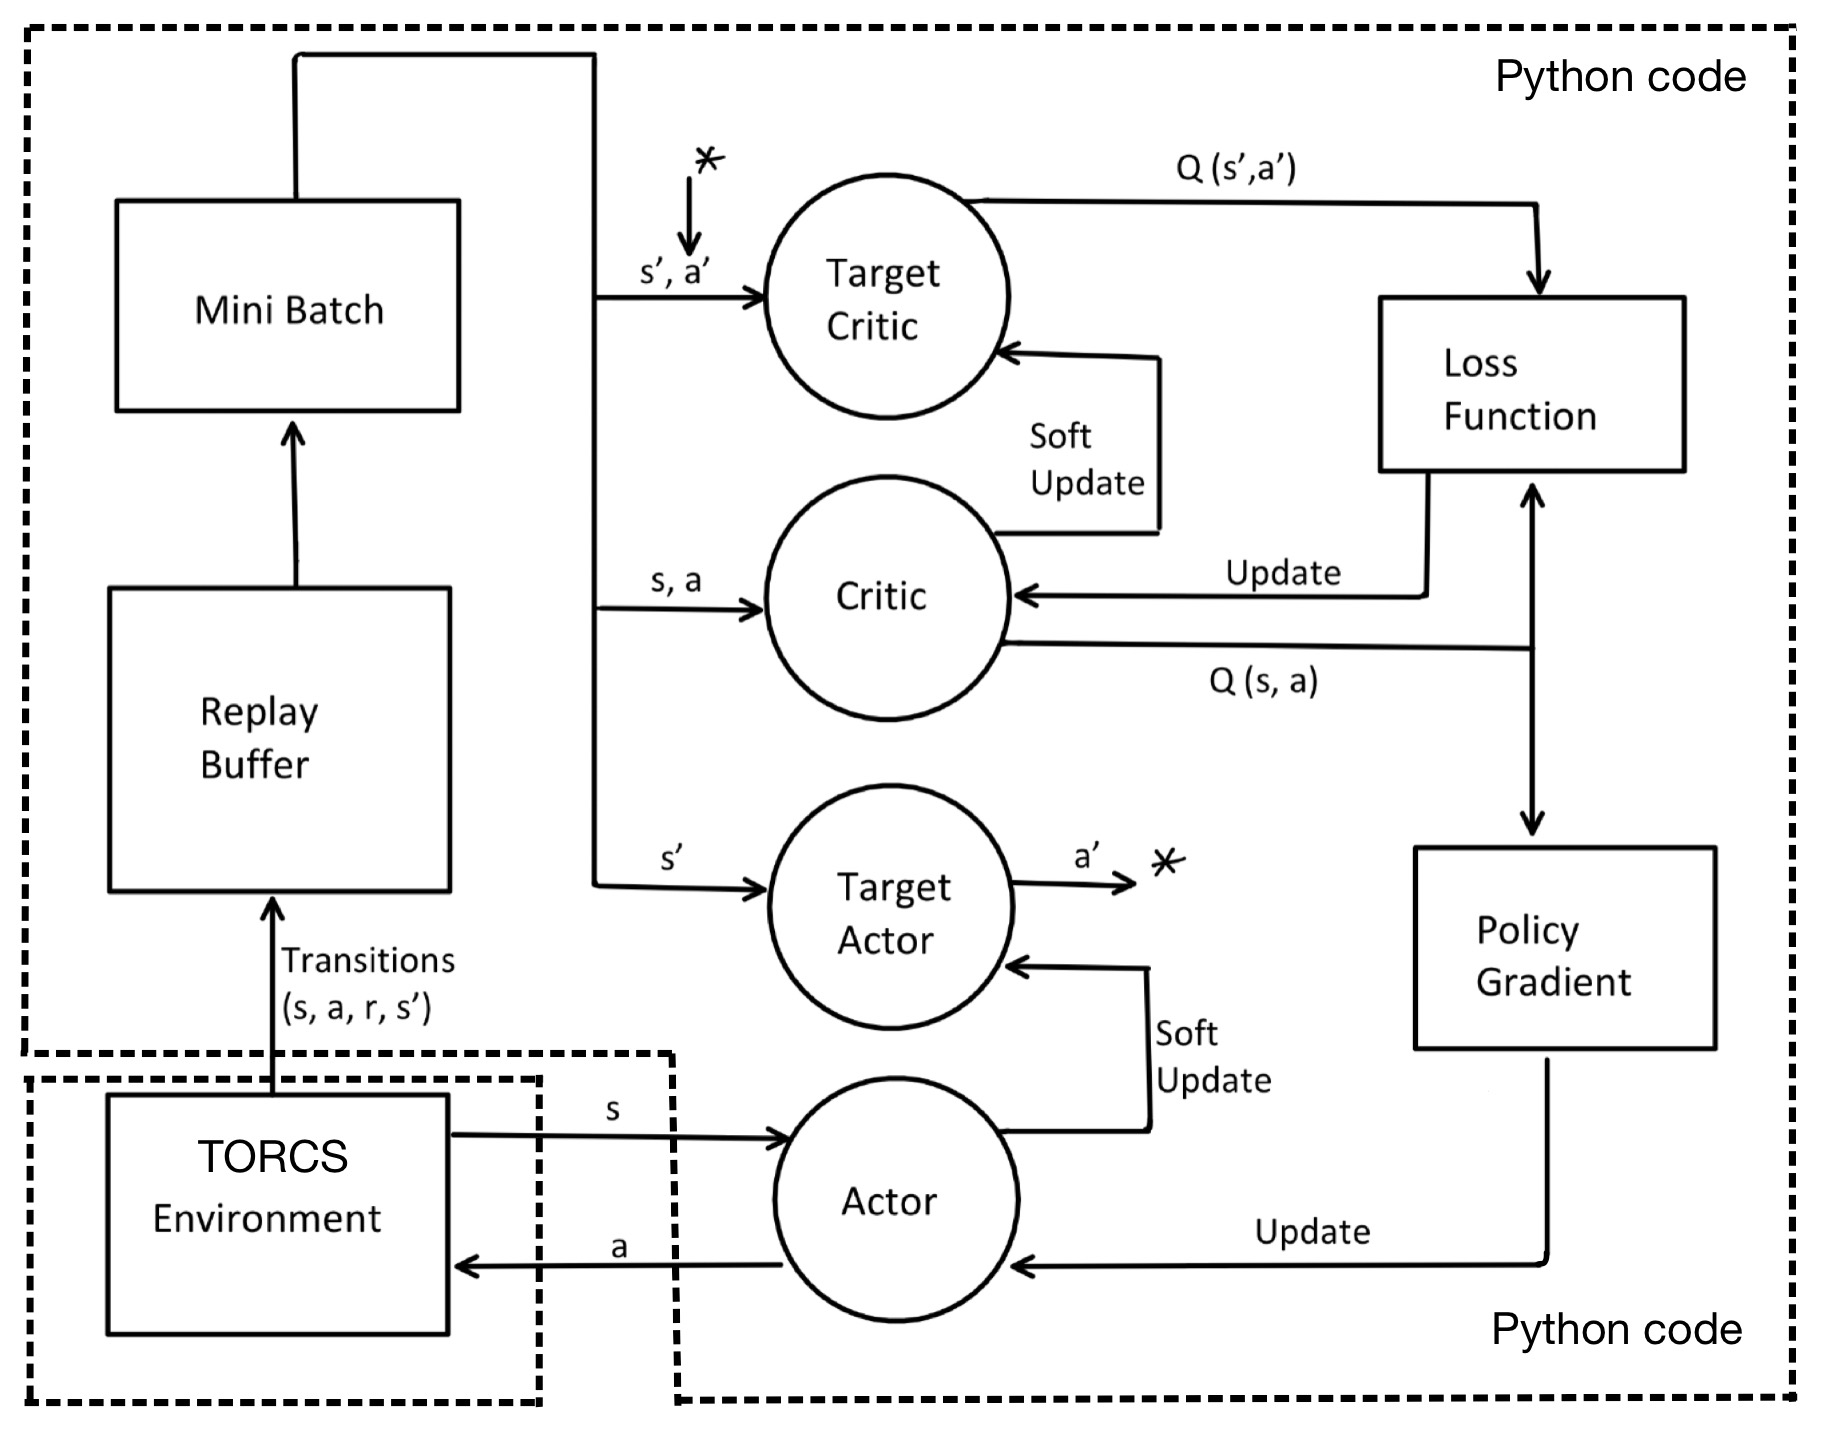
\includegraphics[width=0.9\textwidth]{fig19}
	\caption{Deep Deterministic Policy Gradient block diagram  }
	\label{fig:ddpg}
\end{figure}


\begin{algorithm}
	\caption{DDPG Algorithm}\label{alg:cap}
	\begin{algorithmic}[1]
		
		\STATE Ramdomly initialize critic network $Q(s,a|\theta^Q)$ and actor $\mu(s|\theta^\mu)$ with weights $\theta^Q$ and $\theta^\mu$
		\STATE Initialize target network $Q'$ and $\mu'$ with weights $\theta^{Q'} \gets \theta^Q$, $\theta^{\mu'} \gets \theta^\mu$
		\STATE Initialize replay buffer R
	    \FOR{episode = 1, M}
			\STATE Initialize a random process $N$ for action exploration
			\STATE Receive initial observation state $s$
			\FOR{t=1, T}
				\STATE Select action $a_t = \mu(s_t|\theta^\mu) + N_t$ according to the current policy
				\STATE Execute action $a_t$ and observe reward $r_t$ and observe new state $s_{t}^{'}$
				\STATE Store transition $(s_t, a_t, r_t, s_{t}^{'})$ in $R$
				\STATE Sample a random minibatch on $N$ transitions $(s_t, a_t, r_t, s^{'}_{t})$ from $R$
				\STATE Set $y_i = r_i$ + $\gamma Q^{'}(s^{'}, \mu^{'}(s^{'}|\theta^{\mu'})|\theta^{Q'})$
				\STATE Update critic by minimizing the loss: $L = \frac{1}{N} \Sigma_i(y_i - Q(s_i, a_i|\theta^Q))^2$
				\STATE Update the actor policy using the sampled policy gradient:
					\[ \nabla_{\theta\mu} J \approx \frac{1}{N} \Sigma_i \nabla_a Q(s,a|\theta^Q)|_{s=s_i, a=\mu(s_i)} \nabla_{ \theta\mu} \mu(s|\theta^\mu)|_{s_i}\]
				
				\STATE Update the target networks:
					\[ \theta^{Q'}  \gets \tau\theta^Q + (1 - \tau)\theta^{Q'}\]
					\[ \theta^{\mu'}  \gets \tau\theta^\mu + (1 - \tau)\theta^{\mu'}\]
			\ENDFOR
		\ENDFOR
					
	


		
		
	\end{algorithmic}
\end{algorithm}

Initially when the simulator execution is started, the agent is in a new state represented by $s$. It sends its state to the actor. The actor decides the best possible action $a$ and sends it back to the agent. Since agent cannot decide anything on its own, it follows the actions sent by the actor. After implementing the action, it gets a reward $r$ (which can be anything depending upon how good the action was) and goes to a new state $s'$. The entire transition comprising of $(state \ s, action \ a, reward \ r, new \ state \ s')$ is stored in a replay buffer. From this buffer, random sampling is done and a few transitions are stored in a mini batch. The state $s$ and action $a$ are then sent to the critic to evaluate the action taken by the actor. The critic generates a Q value for the state-action pair and this value shows how good the action was for that particular state. From the mini batch, the next state $s'$ is sent to the target actor. Target actor is expected to give the action $a'$ that is most suitable for the next state $s'$. This next state $s'$ and next action $a'$ is then sent to target critic. The role of target critic is to evaluate the action $a'$ that was recommended by the target actor for the state $s'$ and generate a Q value for $(s', a')$ pair. Using the Q values for both $(s', a')$ and $(s, a)$ pairs, the loss function is calculated which is used to update the critic network. This helps the critic evaluate actor's actions in a better way. Furthermore, the Q value of $(s, a)$ is used to calculate the policy gradient which is in turn used to update the actor network. This helps the actor to make improved decisions. Target networks are not updated with calculated values. Instead, a soft update is carried out after the actor and critic networks are updated. Soft update involves updating the target network by a very small factor called $\tau$ with a typical value being 0.001. Once all these steps are carried out, the agent would have reached a new state and the cycle continues. The actor makes use of neural network to calculate the desirable action $a$ whereas the critic uses neural network to compute Q values \cite{lillicrap2015continuous}. 



 
\subsection{State Space}
The state space consists of velocity of the car, tangential angle of the car with respect to road, horizontal distance between the centre of the lane and car, distance between lane edge and agent, distance between the agent and vehicles ahead, and on the right side of the agent.
According to the agent state, the actor network encodes a state to action at time t. This action is sent to the simulator through shared memory to control the car and return the next state, reward for the same. In each iteration, the set $\langle state, action, reward, next\_state \rangle $
is collected and is stored into the replay buffer for network training. The velocity vector of the car is divided into three orientations x, y, z 
$\epsilon R^3$. The offset $\delta \epsilon R^1$ is the distance between the agent and centre of the track is normalized between (\ -1, 1)\ . The distance between the agent and the edge of the lane $\zeta \epsilon R^{19}$ is measured in (\-45, -19, -12, -7, -4, -2.5, -1.7, -1, -0.5, 0.5 ,1 , 1.7, 2.5 , 4 , 7, 12, 19, 45)\ degrees with respect to front of the agent. The parameter $\theta  \epsilon R^1 $ is angle between direction of the track and direction of the agent and it is measured in radians between (\ $ -\pi, \pi$). 
These values are as shown in Figure \ref{fig:envt} and Table \ref{table:1}. 
DistF and DistR are two variables that define the distance between the agent and obstacles at the front and at the right side respectively. Since 4 sensors spread across the front of the agent simultaneously detect for obstacles ahead  upto a distance of 200 metres, DistF consists of a set of 4 values. DistR consists of a set of 14 values with maximum range of 200 metres as 14 sensors, that are located on the right side of the agent, are used to detect obstacles on the right side.



\begin{figure}[h]
	\centering
	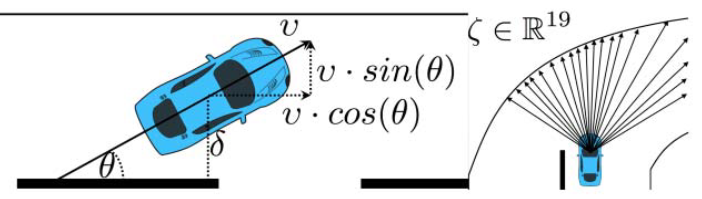
\includegraphics[width=0.7\textwidth]{fig4}
	\caption{Driving Environment \cite{huang2019end} }
	\label{fig:envt}
\end{figure}

%\begin{center}

\begin{table}[h]
	\centering
	\caption{Table of States \cite{huang2019end} }
	\smallskip
	\begin{tabular}{ |p{3cm}|p{6cm}|p{3cm}|  }
		
		\hline
		\textbf{States Symbol}  & \textbf{Description}  &\textbf{Range} \\
		
		\hline
		\hline
		$v (km/h ) $ & Agent's velocity &$ (0, 300) \epsilon R^3 $ \\
		\hline
		$\delta$ & Offset between centre of the lane and the agent horizontally   & $(-1, 1) \epsilon R^1 $ \\
		\hline
		$\theta ( radian ) $ &Departure angle between the lane and agent & $(-\pi, \pi) \epsilon R^1$ \\
		\hline
		$\zeta(m) $  &Distance between edge of the lane and agent & $(0, 200) \epsilon R^{19} $ \\
		
		\hline
		$DistF (m) $  &Distance between the agent and obstacle(s) ahead of it & $(0, 200) \epsilon R^{4} $ \\
		
		\hline
		$DistR(m) $  &Distance between the agent and obstacle(s) on the right side & $(0, 200) \epsilon R^{14} $ \\
		
		\hline
	\end{tabular}
	
	%\end{center}
	\label{table:1}
\end{table}

\subsection{Action Space}

Agent action space $a_t = (\ accelerate, brake, steer )\ $ represents agent acceleration, braking, and steering angle
respectively as illustrated in Table \ref{table:2} in detail.
Acceleration value of 1 implies that the agent has applied full throttle i.e. in human driving terminology, it has pressed the accelerator pedal completely. If acceleration value is 0, it implies that the agent has completely let go of the accelerator pedal and it is moving only due to its momentum. 
Brake value of 0 states that the brake pedal is not at all pressed and a value of 1 imples that it is completely pressed. 
Steering value of -1 represents full right and +1 represents full left turn.  
\\
\begin{table}[h]
	\centering
	\caption{Table of Actions \cite{huang2019end}}
	\smallskip
	\begin{tabular}{ |p{3.1cm}|p{6cm}|p{3cm}|  }
		
		\hline
		\textbf{Action Symbol}  & \textbf{Description}  &\textbf{Range} \\
		
		\hline
		\hline
		accelerate & Current acceleration &$ (\ 0, 1)\ \epsilon R^1 $ \\
		\hline
		brake & Current braking   & $(\ 0, 1)\ \epsilon R^1 $ \\
		\hline
		steer &Current steering angle: negative for right, positive for left & $(\ -1, 1)\ \epsilon R^1$ \\
		\hline
		
	\end{tabular}
	
	%\end{center}
	\label{table:2}
\end{table}

\subsection{Reward Function }

One of the major tasks is designing an appropriate reward function. This function needs to be properly adjusted so that the car knows its priorities well and drives in a controlled manner. To briefly explain a scenario, consider an autonomous car X which is steadily going in its lane. It is getting some positive reward. Suppose X detects some other car, named Y, which is seemingly rushing towards X and it might end up crashing onto the car X, then ego-car (X) must receive higher rewards if it decides to take an action of applying brake and maneuvering it away from Y. In order to achieve the objective of lane keep, the car needs to be trained with altered reward function wherein it must get a higher reward for staying in its lane and a lesser reward for swerving away from the required lane. Another possible approach here is to make use of the sensors to limit the car in one lane thereby creating a pseudo boundary for the car. 

The current reward function is $R = v cos(\theta) - v sin(\theta) - v |\delta|$ where $\theta$ is the departure angle, $v$ is the speed of the agent and $\delta$ is the offset between agent and centre of lane as shown in Figure \ref{fig:envt}. If the departure angle is less, then $cos(\theta)$ will be high while $sin(\theta)$ will be a minute value. If the agent is near the centre of the lane, only a small value will be subtracted. In case it is near the edge of the lane, a higher value will be subtracted from the reward function. The second part of the work involves detection of obstacle using sensors. Two different sensors are used for this process, namely \emph{opponents} and \emph{track}. The \emph{track} sensor is as represented by the $\zeta$ value which is shown in Table \ref{table:1}. It consists of 19 range-finder sensors which contain the distance between the centre of the car and edge of the lane. These sensors are stored in a python list in the implementation. The 36 range-finder values given by the \emph{opponents} sensor are also stored in a python-list. These are located throughout the car at every 10 degrees and they have a maximum range of 200 metres. In case no other cars are present, this sensor outputs the maximum value i.e. 200 metres from each of the sensors. Otherwise it sends the distance between the agent and other cars present on track. 

\section{Implementation}

\subsection{Lane Keep}
This is the primary objective of this project. Here, \emph{trackPos} sensor is used to implement the lane keep operation. Whenever the agent is in a new state, the \emph{trackPos} sensor outputs a value which defines the relative position of the agent on the track. It is represented by the greek symbol $\delta. $ 

%If it is driving exactly at the centre of the track (i.e. it is occupying portions of both the lanes), \emph{trackPos} will give a value of 0. 

In case the agent is driving on the left edge of the left lane, \emph{trackPos} sensor outputs a value of +1 and similarly if it is on the right edge of the left lane, the sensor outputs a value of -1. If the car needs to be at the centre of the left lane, it must be constantly maintaining a value of around 0. Of course, it cannot maintain driving at the centre of the lane at all times. Owing to some tight corners, it does deviate from the centre a bit.

There are two methods implemented in this work to enable lane keep. The first one is a part of the reward function. The third term in the reward function is $v|\delta|$. If the agent is driving at the centre of the lane, $\delta$ will be almost close to 0. In case it has deviated a lot from the centre, $v|\delta|$ a considerbly large value, will be subtracted from the reward function. When the reward has reduced, the agent learns that it is not the optimal path to follow and tries to increase the same by diligently following the lane in the future. The first method is very efficient in teaching the agent to drive in the centre of its lane. However, the second approach is also implemented to leave no room for error. In this method, a pseudo boundary is created between +0.2 and -0.2 corresponding to the \emph{trackPos} sensor. If the agent's \emph{trackPos} value is greater than +0.2, it means that the agent is steering left from the centre of the lane. Hence the \emph{steer} value is negated to enable the agent go steer back to the centre of the lane. If the value is lesser than -0.2, it signifies that the agent is steering right from the centre of the lane. Just like it was done earlier, the \emph{steer} value is negated so that the agent can steer back to the centre of the lane. 

\subsection{Front obstacle detection}


Though the simulator gives the freedom of implementing both Left Hand Drive(LHD) and Right Hand Drive(RHD), the former driving style was chosen as it is more common around the world. Four sensors out of the 36 \emph{opponents} sensors are used for front obstacle detection. 
Whenever the car enters a new state, it waits for a few millisecond to receive instructions from actor network on how to proceed. During this time interval, all the sensor readings are collected and analysed to see if any obstacles are present ahead of the vehicle. If any obstacle is detected beyond 50 metres, it is not required to apply brakes as there is ample distance between the agent and the obstacle. In case front \emph{opponents} sensors detect a car within a range of 30-50 metres ahead, the agent stops accelerating i.e. directly sets its value to 0. Setting the value directly to zero is analogous to taking the foot off the accelerator pedal in real world driving scenario. At this point the agent keeps moving due to its momentum and gradually slows down due to friction. After a few seconds, if the obstacle ahead is less than 30 metres, it applies brakes slightly i.e. it sets the brake value to 0.3 as this is the ideal value to gradually slow down the vehicle. If the value is greater than 0.3, the braking action will involve jerky motion but if it is less than 0.3, it may not slow down at the desired rate. If the obstacle is less than 20 metres away, it applies brakes a tad bit stronger with a value of 0.7. At this value, the vehicle reduces the speed quickly as the obstacle is not very far and if it does not apply brakes with this value, the agent might end up very close to the obstacle with a considerably higher speed after which collision is inevitable. In case the obstacle is less than just 10 metres away, it applies full brakes i.e. sets brake value to 1, so that it comes to a complete halt. 
If the obstacle is detected early enough, braking action is done in a step by step manner over a distance of 50 metres and it smoothly comes to a halt. 
In case the obstacle suddenly comes in the path of the agent with less distance between them, then the agent applies full brake inorder to avoid collision. In such a scenario, braking will not be smooth but that is secondary since it is more important to avoid collision. 

\subsection{Overtaking}
This is interconnected with front obstacle detection. When driving in a lane and any obstacle appears suddenly, the only thing that comes to the mind of any driver is to apply the brakes and stop swiftly and that is exactly what the agent does too. On the other hand, if an obstacle is detected well in advance, the agent can plan to overtake the same. When the distance between the agent and the vehicle ahead is around 20 metres, agent takes another set of \emph{opponents} sensor readings to check if there are any vehicles that are currently on the right lane. It uses the same sensor to detect the cars on the right lane that it used to detect the cars or obstacle ahead of it. If it is clear of any traffic, it steers to the right lane. After overtaking a vehicle, it checks if it can come back to its previous lane. If the path is again clear, it steers back to its lane and continues driving. 

The agent's speed is limited to 90 kilometre per hour. While overtaking, imagine a scenario where the agent has completed half of the overtaking process by going to the right lane. At this point, if the vehicle which was being overtaken, suddenly increases its speed and if this is equal to or more than the speed of the agent, the agent decides to abort the overtaking procedure. The agent cannot measure the speed of other vehicles, instead it knows that other vehicle's speed has increased when it senses that it is driving paralelly at its maximum speed with the vehicle that it just tried to overtake. At such a scenario, it slows down a little by setting the acceleration value to zero and checks if it can go back to its previous lane. If the road is clear, it steers left and follows the car which it had intended to overtake. 

\subsection{Side obstacle detection}
To detect the obstacles at the sides of the agent, a total of 28 sensors are utilized. If all the vehicles that are plying over a stretch of road meticulously follow their lane, then agent takes no action. However if any vehicle deviates from its lane and enters the lane that belongs to the agent, at that time the problems arise. If the agent senses any vehicle approaching very close to it from sides, it slightly steers away to avoid collision. It moves away from the approaching vehicle only if there is space left on the road. In case it was already driving on the edge of the road and if some vehicle approaches from sides, then it slowls down letting the other vehicle pass. If such a situation occurs in the real world, drivers first press the horns of their vehicle to alert the driver who is deviating from their lane. Since the simulator does not have that privilege, it simply slows down as that is the best the agent can do to avoid a sideward collision.









